\newcommand{\Bels}{\Xi}
\newcommand \Params {\Theta}
\renewcommand \param {\theta}
\newcommand \marg {\phi}

% \newcommand \Bay {\ensuremath{\mathscr{B}}}
% \newcommand \Adv {\ensuremath{\mathscr{A}}}


\section{Bayesian inference and privacy}
\begin{frame}
  \frametitle{Bayesian inference and differential privacy}
  \begin{block}{Bayesian estimation}
    \begin{itemize}
    \item What are its robustness and privacy properties?
    \item How important is the selection of the prior?
    \end{itemize}
  \end{block}

  \begin{block}{Limiting the communication channel}
    \begin{itemize}
    \item How should we communicate information about our posterior?
    \item How much can an adversary learn from our posterior?
    \end{itemize}
  \end{block}

\end{frame}

\subsection{Setting}
\begin{frame}
  \begin{block}{Dramatis personae}
    \begin{itemize}
    \item $x$ -- data.
    \item $\Bay$ -- a (Bayesian) statistician.
    \item $\bel$ -- the statistician's prior belief.
    \item $\param$ -- a parameter
    \item $\Adv$ -- an adversary. He knows $\bel$, should not learn $x$.
    \end{itemize}
  \end{block}
  \uncover<2>{
    \begin{block}{The game}
      \begin{enumerate}
      \item \Bay{} selects a model family ($\family$) and a prior
        ($\bel$).
      \item \Bay{} observes data x and calculates the posterior
        $\bel(\param | x)$.
      \item \Adv{} queries  \Bay{}.
      \item \Bay{} responds with a function of the posterior $\bel(\param | x)$.
      \item Goto 3.
      \end{enumerate}
    \end{block}
  }
\end{frame}
\begin{frame}
  \frametitle{Two related problem viewpoints}
  \begin{block}{Bayesian inference view}
    \begin{tikzpicture}
      \node[hidden] at (0,0) (x) {Data};
      \node[known] at (4,2) (pre) {Prior};
      \node[queried] at (4,0) (post) {Posterior};
      \node at (8,0) (access) {Observer};
      \draw [->] (x) -- (post);
      \draw [->] (pre) --(post);
      \draw [<->] (post) -- (access);
    \end{tikzpicture}
  \end{block}
  \begin{block}{Mechanism design view}
    \begin{tikzpicture}
      \node[hidden] at (0,0) (x) {Data};
      \node[known] at (4,2) (mech) {Mechanism};
      \node[queried] at (4,0) (private) {Query};
      \node at (8,0) (access) {Observer};
      \draw [->] (x) -- (private);
      \draw [->] (mech) --(private);
      \draw [<->] (private) -- (access);
    \end{tikzpicture}
  \end{block}

\end{frame}

\begin{frame}

  \frametitle{Two related problem viewpoints}
  \begin{block}{Bayesian inference view}
    \begin{tikzpicture}
      \node[hidden] at (0,0) (x) {Data};
      \node[known] at (4,2) (pre) {Prior};
      \node[queried] at (4,0) (post) {Posterior};
      \node at (8,0) (access) {Observer};
      \draw [->] (x) -- (post);
      \draw [->] (pre) --(post);
      \draw [<->] (post) -- (access);
    \end{tikzpicture}
  \end{block}

  \begin{itemize}
  \item \Bay{} has a prior belief about how well a drug works.
  \item \Bay{} obtains some data about the drug.
  \item \Bay{}'s conclusion from the data is a posterior belief.
  \item \Bay{}'s communicates its conclusion to an observer which:
    \begin{enumerate}
    \item Must be accurate.
    \item Must not reveal a lot about the data.
    \end{enumerate}
  \end{itemize}
\end{frame}


\begin{frame}
  \frametitle{Two related problem viewpoints}
  \begin{block}{Mechanism design view}
    \begin{tikzpicture}
      \node[hidden] at (0,0) (x) {Data}; \node[known] at (4,2) (mech)
      {Mechanism}; \node[queried] at (4,0) (private) {Query}; \node at
      (8,0) (access) {Observer}; \draw [->] (x) -- (private); \draw
      [->] (mech) --(private); \draw [<->] (private) -- (access);
    \end{tikzpicture}
  \end{block}
  \begin{itemize}
  \item We want to design a mechanism.
  \item The observer can ask queries.
  \item The mechanism responds with a response that:
    \begin{enumerate}
    \item Is useful.
    \item Does not reveal a lot about the data.
    \end{enumerate}
  \end{itemize}
\end{frame}


\begin{frame}
  \frametitle{Two related problem viewpoints}
  \begin{block}{Bayesian inference view}
    \begin{tikzpicture}
      \node[hidden] at (0,0) (x) {Data};
      \node[known] at (4,2) (pre) {Prior};
      \node[queried] at (4,0) (post) {Posterior};
      \node at (8,0) (access) {Observer};
      \draw [->] (x) -- (post);
      \draw [->] (pre) --(post);
      \draw [<->] (post) -- (access);
    \end{tikzpicture}
  \end{block}
  \begin{block}{Mechanism design view}
    \begin{tikzpicture}
      \node[hidden] at (0,0) (x) {Data};
      \node[known] at (4,2) (mech) {Mechanism};
      \node[queried] at (4,0) (private) {Query};
      \node at (8,0) (access) {Observer};
      \draw [->] (x) -- (private);
      \draw [->] (mech) --(private);
      \draw [<->] (private) -- (access);
    \end{tikzpicture}
  \end{block}
  \begin{itemize}
  \item We'll discuss a specific mechanism that provides privacy.
  \item The amount of privacy depends on the prior.
  \end{itemize}
\end{frame}

\subsection{Differential privacy}
\begin{frame}
  \frametitle{Differential privacy}
  A randomised mechanism taking data $x$ as input is basically a
  distribution condition on $x$. So we write:
  \begin{definition}[$\only<2->{(}\epsilon\only<2->{,\delta)}$-differential privacy]
    \label{def:dp-basic}
    $\bel(\cdot \mid x)$ is \emph{$\only<2->{(}\epsilon\only<2->{,\delta)}$-differentially private} if, $\forall x \in \CS \alert{= \CX^n}$, $B \subset \Params$
    \[
    \bel(B \mid x) \leq e^\epsilon \bel(B \mid y)\uncover<2->{ + \delta},
    \]
    for all $y$ in the \alert{hamming-$1$ neighbourhood} of $x$. 
  \end{definition}
  \uncover<3->{
    i.e. neighbouring datasets are statistically indistinguishable wrt the distribution induced by the mechanism.

    \begin{remark}
      A similar definition can be given for computationally indistinguishable distributions.
    \end{remark}
  }
\end{frame}

\begin{frame}
  \frametitle{The necessity of randomness}
  \begin{itemize}
  \item Consider a deterministic mechanism $f : \CS \to \{0,1\}$.
  \item<2-> If there is at least one pair $x, y \in \CS$ such that
    \[
    f(x) = 0, \qquad f(y) = 1.
    \]
    then:
  \item<3-> An adversary \Adv{} wants to guess the real data $x^\star$ and knows that $x^* \in \set{x, y}$ can immediately discover the truth.
  \end{itemize}
\end{frame}

\begin{frame}
  \frametitle{Responding to queries}
  \begin{itemize}
  \item \Bay{} normally responds to queries from \Adv{}.
  \item Queries can be defined equivalently as 
    \begin{enumerate}
    \item Additional inputs to the mechanism.
    \item A utility function submitted by \Adv{} that \Bay{} maximises.
    \item An function submitted by \Adv{} that \Bay{} evaluates.
    \end{enumerate}
  \end{itemize}
\end{frame}

\begin{frame}
  \frametitle{Current differentially private mechanisms}
  \begin{block}{Laplace mechanism}
    Add noise to responses to queries.
    \[
    r = \underbrace{q(x)}_{\textrm{ideal response}} + \underbrace{\omega}_{\textrm{noise}}, \qquad \omega \sim \Laplace(\lambda)
    \]
  \end{block}
  \begin{block}{Exponential mechanism}
    Define a utility function $u(x,r)$ maximised for $u(x, q(x))$ 
    \[
    \underbrace{p(r)}_{\textrm{response probability}} \propto e^{\epsilon u(x,r)} \underbrace{\mu(r)}_{\textrm{base measure}}.
    \]
  \end{block}
  \begin{block}{Other methods}
    \begin{itemize}
    \item Subsample + aggregate
    \item Compressed sensing
    \end{itemize}
  \end{block}
\end{frame}

\begin{frame}
  \frametitle{Bayesian inference}
  \only<1>{
    \begin{block}{Estimating a coin's bias}
      A fair coin comes heads $50\%$ of the time. 
      We want to test an unknown coin, which we think may not be completely fair. 
    \end{block}
  }
  \only<1,2>{
    \begin{figure}[h]
      \centering
      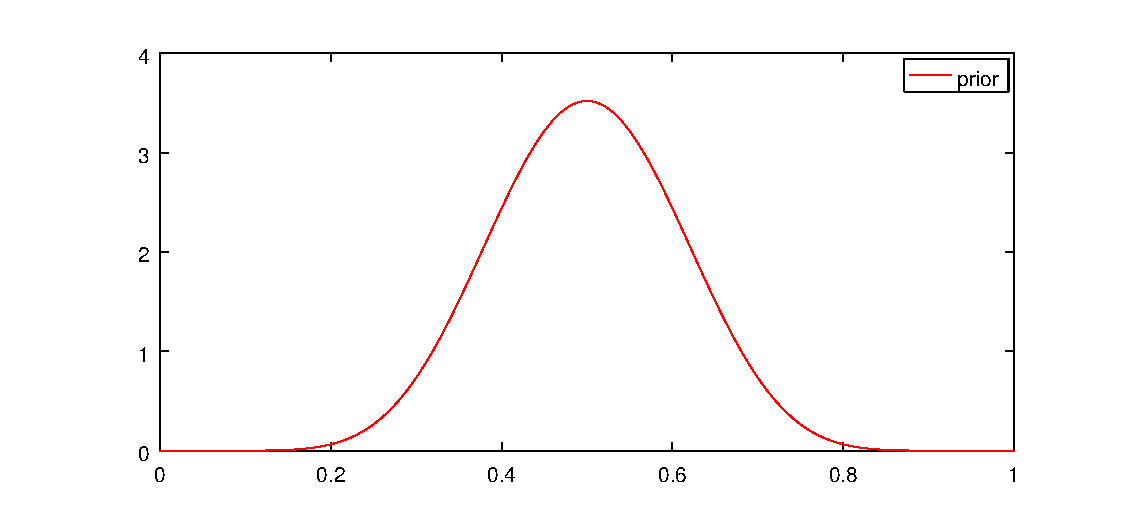
\includegraphics[width=\textwidth]{beta-prior}
      \caption{Prior belief $\bel$ about the coin bias $\theta$.}
    \end{figure}
  }
  \only<2>{
    For a sequence of throws $x_t \in \{0,1\}$,
    \[
    P_\theta(x) \propto \prod_t \theta^{x_t} (1 - \theta)^{1 - x_t}
    = \theta^{\textrm{\#Heads}} (1 - \theta)^{\textrm{\#Tails}}
    \]
  }
  \only<3>{
    \begin{figure}[h]
      \centering
      \includegraphics[width=\textwidth]{beta-likelihood}
      \caption{Prior belief $\bel$ about the coin bias $\theta$ and likelihood of $\theta$ for the data.}
    \end{figure}
    Say we throw the coin 100 times and obtain 70 heads. Then we plot the \alert{likelihood} $P_\theta(x)$ of different models.
  }
  \only<4>{
    \begin{figure}[h]
      \centering
      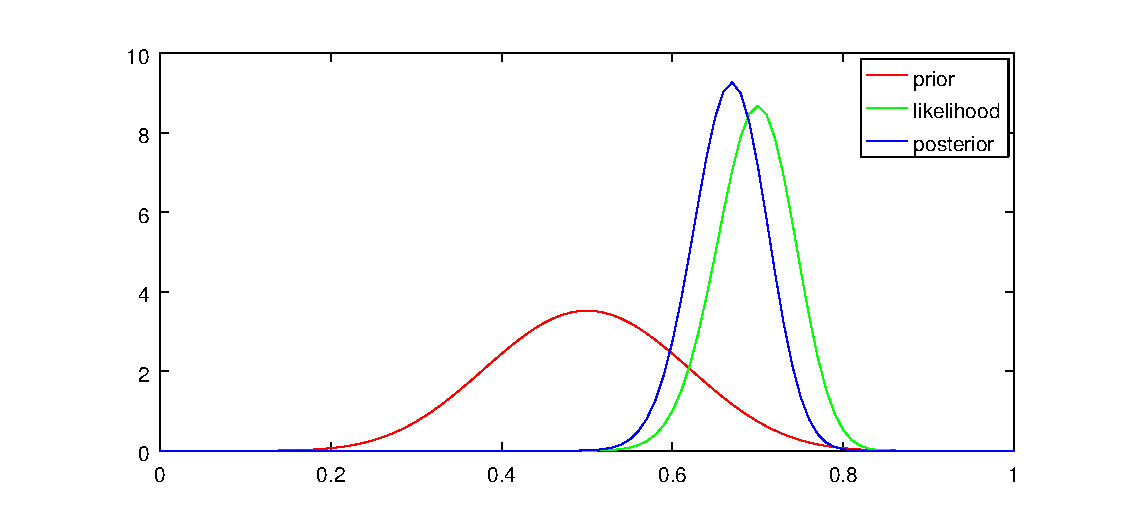
\includegraphics[width=\textwidth]{beta-posterior}
      \caption{Prior belief $\bel(\theta)$ about the coin bias $\theta$, likelihood of $\theta$ for the data, and posterior belief $\bel(\theta \mid x)$}
    \end{figure}
    From these, we calculate a \alert{posterior} distribution over the correct models. This represents our conclusion given our prior and the data.
  }
\end{frame}



\begin{frame}
  \frametitle{Bayesian inference}
  \begin{block}{Setting}
    \begin{itemize}
    \item Dataset space $\CS$.
    \item Distribution family $\family \defn \cset{P_\param}{\param \in \Params}$.
    \item Each $P_\param$ is a distribution on $\CS$.
    \item We wish to identify which $\theta$ generated the observed data $x$.
    \item Prior distribution $\bel$ on $\Params$ (i.e. initial belief)
    \item Posterior given data $x \in \CS$ (i.e. conclusion)
      \begin{align}
        \label{eq:posterior}
        \bel(\param \mid x) &= \frac{P_\param(x) \bel(\param)}{\marg(x)}\tag{posterior}\\
        \marg(x) &\defn \sum_{\param \in \Params} P_\param(x) \bel(\param) \tag{marginal}.
      \end{align}
    \end{itemize}
  \end{block}
  \alert{Standard calculation that can be done exactly or approximately.}
\end{frame}




\section{Bayesian inference for privacy}
\begin{frame}
  \tableofcontents[hideothersubsections]
\end{frame}


\begin{frame}
  \frametitle{What we want to show}
  \begin{itemize}
  \item<1-> If we assume the family $\family$ is well-behaved \ldots
  \item<1-> \ldots or that the prior $\bel$ is focused on the ``nice'' parts of $\family$
  \item<2-> Inference is robust.
  \item<2-> Our knowledge is private.
  \item<2-> There are also well-known $\family$ satisfying our assumptions.
  \end{itemize}
  \uncover<3>{First, we must generalise differential privacy...}
\end{frame}

\begin{frame}
  \frametitle{Differential privacy of conditional distribution $\bel(\cdot \mid x)$}
  \begin{definition}[$(\epsilon, \delta)$-differential privacy]
    \label{def:dp-old}
    $\bel(\cdot \mid x)$ is \emph{$(\epsilon, \delta)$-differentially private} if, $\forall x \in \CS \alert{= \CX^n}$, $B \subset \Params$
    \[
    \bel(B \mid x) \leq e^\epsilon \bel(B \mid y) + \delta,
    \]
    for all $y$ in the \alert{hamming-$1$ neighbourhood} of $x$. 
  \end{definition}
  \uncover<2->{
    \begin{definition}[$(\epsilon, \delta)$-differential privacy under $\xdistChar$.]
      \label{def:dp-new}
      $\bel(\cdot \mid x)$ is \emph{$(\epsilon, \delta)$-differentially private under } a \alert{pseudo-metric} $\xdistChar : \CS \times \CS \to \Reals_+$ if, $\forall B \subset \Params$ and  $x \in \CS$, 
      \[
      \bel(B \mid x) \leq e^{\epsilon \xdist{x}{y}} \bel(B \mid y) + \delta \xdist{x}{y}, \qquad \forall y \in \CS
      \]
    \end{definition}
    \alert{If two datasets $x,y$ are close, then the distributions $\bel(\cdot \mid x)$ and $\bel(\cdot \mid y)$ are also close.}
  }
\end{frame}


\begin{frame} 
  \frametitle{Sufficient conditions}
  \begin{assumption}[$\family$ is Lipschitz]
    For a given $\rho$ on $\CS$, $\exists L > 0$ s.t. $\forall \param \in \Params$:
    \begin{align}
      \left|\ln \frac{P_\param(x)}{P_\param(y)}\right|
      &\leq
        L \xdist{x}{y}, \qquad \forall x, y \in \mathcal{\CS},
        \label{eq:hoelder-observations}
    \end{align}  
    \label{ass:hoelder-observations}
  \end{assumption}
  \only<1>{
    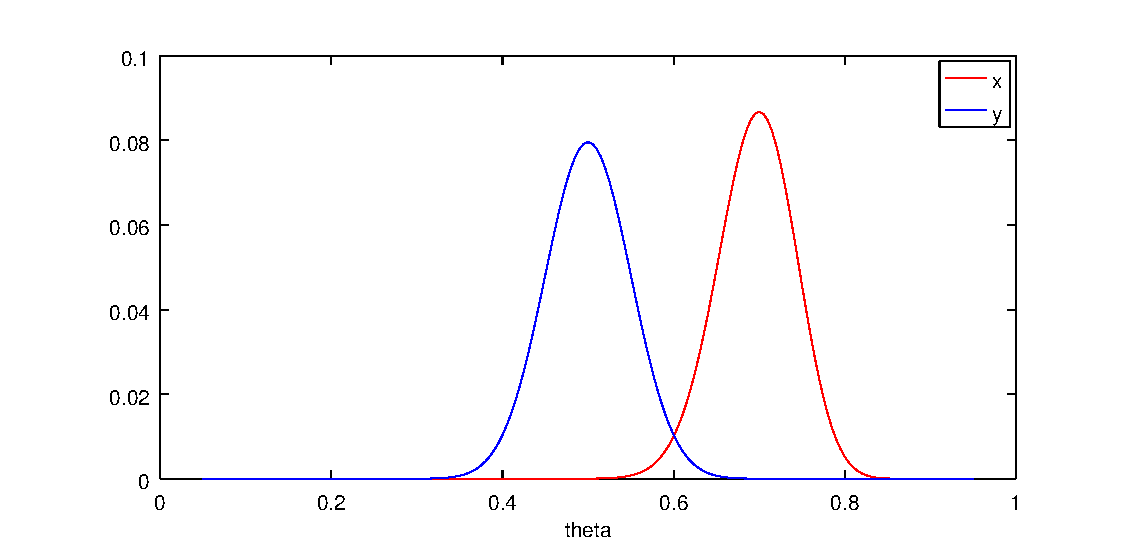
\includegraphics[width=\textwidth]{beta-lipschitz}
  }
  \only<2>{
    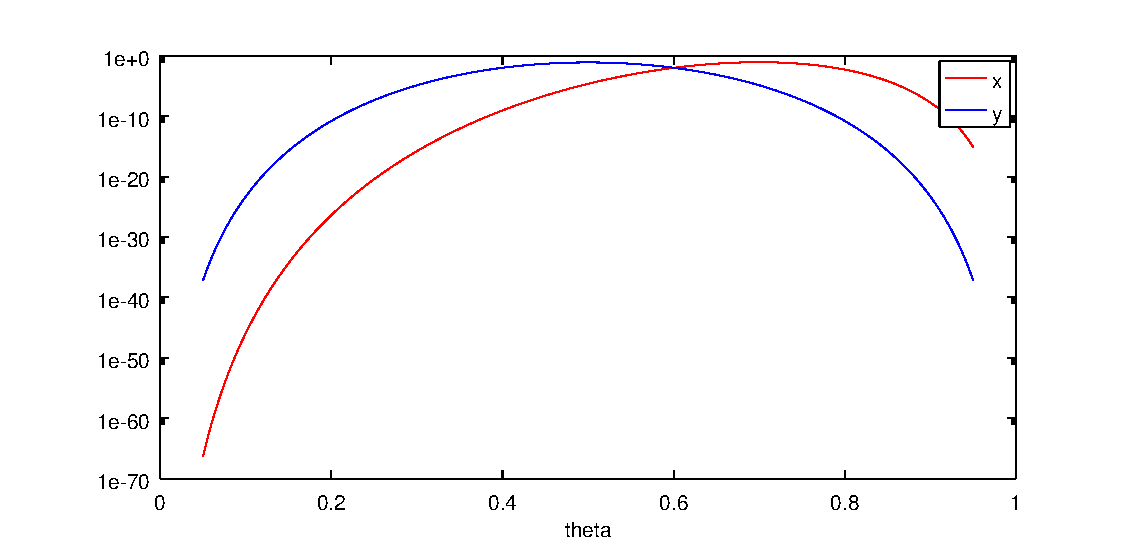
\includegraphics[width=\textwidth]{beta-log-lipschitz}
  }
\end{frame}


\begin{frame}
  \frametitle{Stochastic Lipschitz condition}
  \begin{assumption}[The prior is concentrated on nice parts of $\family$]
    Let the set of $L$-Lipschitz parameters be $\Theta_L$.
    Then $\exists c \constg > 0$ s.t. 
    \begin{equation}
      \bel(\Params_L) \geq 1 - \constg \exp(-cL), \forall L
    \end{equation}
    \label{ass:hoelder-measure-observations}
  \end{assumption}
  \only<1>{
    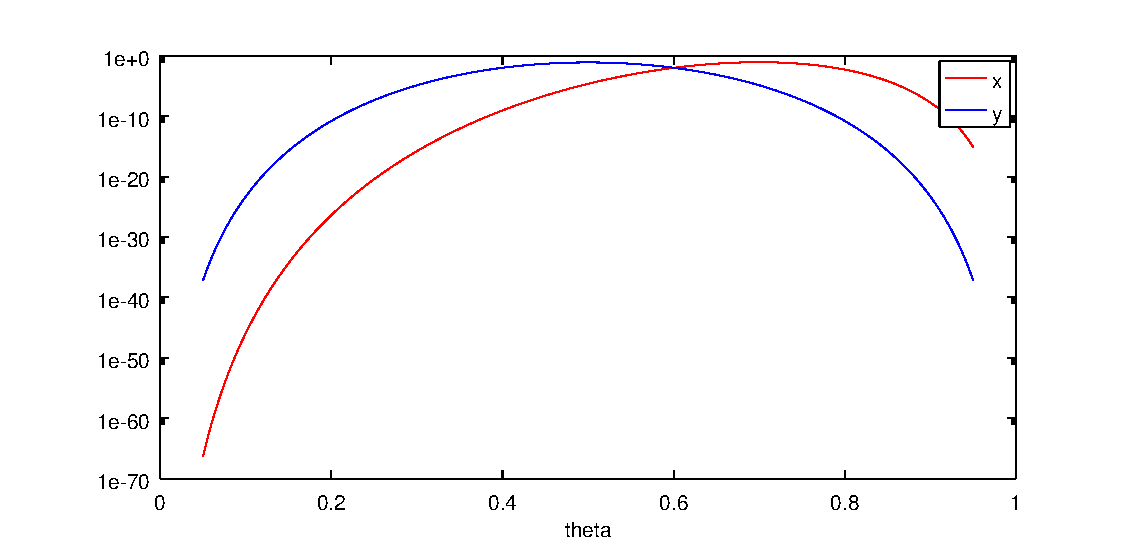
\includegraphics[width=\textwidth]{beta-log-lipschitz}
  }
  \only<2>{
    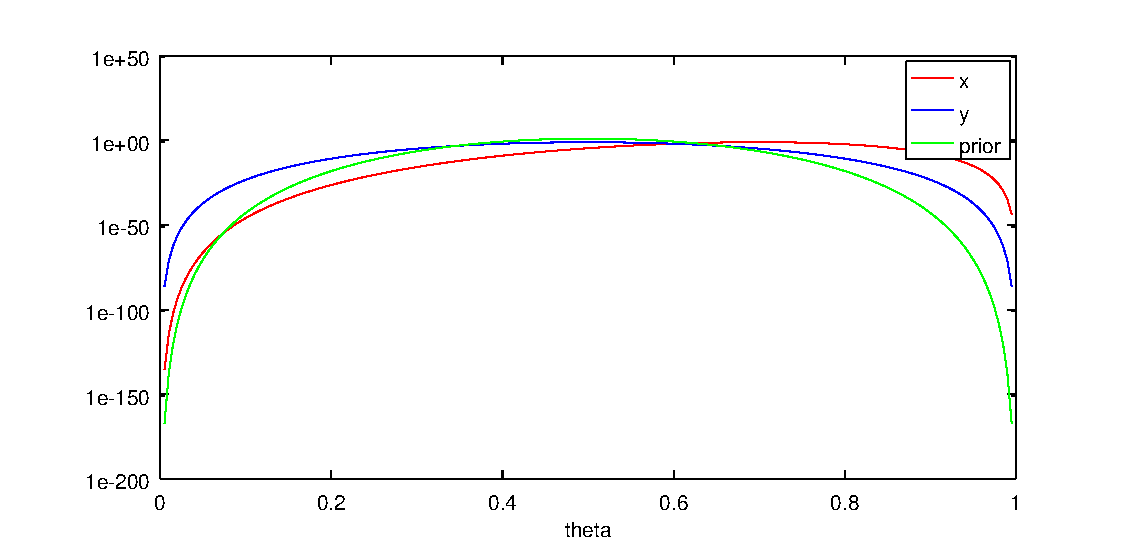
\includegraphics[width=\textwidth]{beta-log-lipschitz-prior}
  }
\end{frame}

\iffalse
\begin{frame}
  \frametitle{Necessary condition}
  To achieve differential privacy, the metric must be based on a \alert{Bayesian sufficient statistic $\tau$}
  \[
  \xdist{x}{y} = \norm{\tau(x) - \tau(y)},
  \]
  such that $\xdist{x}{y} = 0$ implies that
  \[
  \bel(B \mid x) = \bel(B \mid y).
  \]
\end{frame}
\fi


\subsection{Robustness and privacy of the posterior distribution}
\label{sec:robustness}
\begin{frame}
  \frametitle{Robustness of the posterior distribution}
  \begin{definition}[KL divergence]
    \begin{equation}
      \label{eq:kl-divergence}
      \dist{P}{Q} \defn \int \ln \frac{\dd{P}}{\dd{Q}} \dd{P}.
    \end{equation}
  \end{definition}
  \begin{theorem}
    \begin{enumerate}[(i)]
    \item<2-> Under Assumption~\ref{ass:hoelder-observations},
      \begin{equation}
        \dist{\bel(\cdot \mid x)}{\bel(\cdot \mid y)}
        \leq
        2L\xdist{x}{y}
      \end{equation}
      \label{the:kl-1}
    \item<3-> Under Assumption~\ref{ass:hoelder-measure-observations},
      \begin{equation}
        \dist{\bel(\cdot \mid x)}{\bel(\cdot \mid y)}
        \leq
        \frac{\kappa C_\bel }{c} \cdot 
        \xdist{x}{y}
      \end{equation}
      \label{the:kl-2}
    \end{enumerate}
    \label{the:kl}
  \end{theorem}
\end{frame}

\begin{frame}
  \frametitle{Differential privacy of the posterior}
  \begin{theorem}
    \begin{enumerate}
    \item<1-> Under Assumption~\ref{ass:hoelder-observations}, 
      $B \in \fields{\Params}$:
      \begin{align}
        \bel(B \mid x) & \leq e^{ 2L \xdist{x}{y}} \bel(B \mid y) 
      \end{align}
      \ie the posterior is $(2L, 0)$-DP under $\xdistChar$.
      \label{thm:dp1}
    \item<2-> Under Assumption~\ref{ass:hoelder-measure-observations}, for
      all $x,y \in \mathcal{\CS}$, $B \in \fields{\Params}$:
      \begin{align*}
        \abs{\bel(B \mid x) - \bel(B \mid y)}
        & \leq \sqrt{\frac{\constScaleB C_\bel }{2c} \xdist{x}{y}}
      \end{align*}
      \ie the posterior is $\left(0,  \sqrt{\frac{\constScaleB C_\bel }{2c}}\right)$-DP under $\sqrt{\xdistChar}$.
      \label{thm:dp2}
    \end{enumerate}
    \label{thm:dp}
  \end{theorem}
\end{frame}

\subsection{Posterior sampling query model}

\begin{frame}
  \frametitle{Posterior sampling query model}
  \begin{itemize}
  \item<1-> We select a prior $\bel$.
  \item<1-> We observe data $x$.
  \item<1-> We calculate a posterior $\bel(\cdot \mid x)$.
  \item<1-> An adversary has sampling-based access to the posterior.
  \end{itemize}

  \uncover<2->{
    \begin{block}{First idea}
      At time $t$, the adversary observes a \alert{sample} from the posterior:
      \[
      \param_t \sim \bel(\param \mid x),
      \]
    \end{block}
  }
  \uncover<3->{
    $\Adv$ may instead \alert{query} using a function $q : \Theta \to \CR$, to obtain:
    \[
    r_t = q(\theta_t)
    \]
  }
  \uncover<4->{
    \begin{block}{Avoiding disclosure with multiple queries}
      We simply release $n$ samples from the posterior
      \[
      \param_t \sim \bel(\param \mid x), \qquad t \in \set{1, \ldots, n}
      \]
    \end{block}
  }
\end{frame}

\begin{frame}
  \frametitle{Responding to queries via utilities}
  \begin{block}{Posterior sampling}
    Given a prior $\bel$, data $x$ and number of samples $n$,
    \[
    \hat{\Params} \sim \bel^n( \cdot \mid x).
    \]
  \end{block}
  \begin{block}{Sample query response}
    For a query $q_t$ and utility function $u_\param : \CR \times \CQ \to [0,1]$, return:
    \[
    r_t \in \argmax_r \sum_{\param \in \hat{\Params}} u_\param(r, q_t)
    \]
  \end{block}
  \begin{theorem}
    If $\bel^\star$ is \Adv{}'s preferred prior, and we restrict it so  $\bel(\Params_L) = 1$:
    \begin{enumerate}[(a)]
    \item The algorithm is $2 L n$-differentially private.
    \item \Adv{}'s regret is  $O([1 - \bel^\star(\Params_L)] + \sqrt{\ln (1/\delta)/n})$, w.p. $1 - \delta$.
    \end{enumerate}
  \end{theorem}
\end{frame}

\begin{frame}
  \frametitle{Another look at the exponential mechanism}
  Define a utility function $u(x,r)$
  \[
  p(r) \propto e^{\epsilon u(x,r)} \mu(r).
  \]
  Respond with $r$ with probability $p(r)$.


  \begin{block}{Connection to posterior mechanism}
    \begin{itemize}
    \item Responses are parameters $\theta$.
    \item Take $u(\theta,x) = \log P_\theta(x)$.
    \item Take $\mu(\theta) = \bel(\theta)$.
    \item Then $p(\theta) = \bel(\theta \mid x)$.
    \item Rather than tuning $\epsilon$, we can tune 
      \begin{itemize}
      \item The prior $\bel$.
      \item The number of samples $n$.
      \end{itemize}
    \end{itemize}
  \end{block}
\end{frame}

\begin{frame}
  \frametitle{Reduction of privacy to a testing problem}
  \uncover<1->{
    \begin{alertblock}{How many samples $n$ should we release?}
      \begin{itemize}
      \item Different datasets $x, y$ give different $\bel(\cdot \mid x), \bel(\cdot \mid y)$.
      \item How many samples are needed to differentiate them?
      \end{itemize}
    \end{alertblock}
  }

  \uncover<2->{
    \begin{theorem}
      Under Assumption~\ref{ass:hoelder-observations}, the adversary can distinguish between data $x, y$ with probability $1 - \delta$ if:
      \begin{equation}
        \xdist{x}{y} \geq \frac{3}{4L \alert{n}} \ln \frac{1}{\delta}.
      \end{equation}
      Under Assumption~\ref{ass:hoelder-measure-observations}, this becomes:
      \begin{equation}
        \label{eq:adversary-sample-complexity-2}
        \xdist{x}{y} \geq \frac{3 c}{2 \constScaleB C_\bel \alert{n}} \ln \frac{1}{\delta}.
      \end{equation}
      \label{the:adversary-sample-complexity}
    \end{theorem}
  }
\end{frame}



\begin{frame}
  \frametitle{The Le Cam method for lower bounds}
  Idea: Use $\CS$ for the ``parameter'' space of an estimator.
  \uncover<2->{
    \begin{block}{The family of posterior measures}
      \begin{equation}
        \label{eq:posterior-family}
        \Bels \defn \cset{\bel(\cdot \mid x)}{x \in \CS},
      \end{equation}
    \end{block}
  }
  \uncover<3->{
    \begin{lemma}[Le Cam's method]
      Let $\psi(\param)$ be an estimator of $x$. 
      Let $\CS_1, \CS_2$ be  $2\delta$-separated and say $x \in S_i \Rightarrow \bel(\cdot \mid x) \in \Bels_i \subset \Bels$. Then:
      \begin{align}
        \sup_{x \in \CS} \E_\bel (\xdist{\psi}{x} \mid x) \geq \alert{\delta} \sup_{\bel_i \in \textrm{co}(\Bels_i)} \|\bel_1 \wedge \bel_2\|.
      \end{align}
    \end{lemma}
  }
  \uncover<4->{
    Expected distance between the real and guessed data:
    \[
    \E_\bel (\xdist{\psi}{x} \mid x)
    =
    \int_\Theta \xdist{\psi(\theta)}{x} \dd{\bel}(\theta \mid x),
    \]
  }

\end{frame}

\section{Examples}
\begin{frame}
  \frametitle{When do these assumptions hold?}
  \begin{example}[Exponential families]
    Family $\family$, with sufficient statistic $T$.
    \[
    p_{\param}(x) = h(x) \exp\left\{ \eta_{\param}^{\top} T(x) -
      A(\eta_{\param})\right\}
    \]
    For a given $\param \in \Params$, we want to test if:
    \[
    \left| \ln(h(x)/h(y)) + \eta_{\param}^{\top}\left(T(x)-T(y)\right) \right| \le L \xdist{x}{y}, \qquad \forall x, y \in \mathcal{\CX}
    \enspace.
    \]
  \end{example}
\end{frame}

\begin{frame}
  \begin{example}[Exponential distribution]
    Exponential prior with parameter $c > 0$, satisfies Assumption 2.
  \end{example}

  \begin{example}[Discrete Bayesian networks]
    \[
    \left|\ln \frac{P_\param(x)}{P_\param(y)}\right| \leq \ln \frac{1}{\epsilon} \cdot \xdist{x}{y},
    \]
    where: $\xdist{x}{y}$ is the number of edges and nodes influenced by the differences in $x,y$
    and $\epsilon$ the smallest $P_\theta$-mass placed to any event.
  \end{example}
\end{frame}

\section{Multi-armed bandits}
\begin{frame}
  \frametitle{Multi-armed bandits}
  Using one UCB1-style and one interval-style algorithm, we can obtain DP bandits with regret:
  \[
  O(\epsilon^{-1} \log \log T + \log T), \tag{DP-UCB}
  \]

  \[
  O(\epsilon^{-1} + \log T) \tag{DP-UCB-INT}
  \]
\end{frame}

\section{Experiments}
\begin{frame}
  \frametitle{Discrete Bayesian Networks}
  \includegraphics[width=0.95\linewidth]{figures/DNB_16_var-accuracy-eps}
\end{frame}

\begin{frame}
  \frametitle{Linear regression}
  \includegraphics[width=0.95\linewidth]{figures/lr-mse-samplerate.pdf}
\end{frame}

\begin{frame}
  \frametitle{Multi-armed bandits}
  Regret for $\epsilon = 0.1$, 10 arms

  \scalebox{0.5}{\input{figures/arms_10_eps_01.pgf}}


\end{frame}

\begin{frame}
  \frametitle{Conclusion}
  \begin{itemize}
  \item Bayesian inference is inherently robust and private [hooray].
  \item Privacy is achieved by posterior sampling [Dimitrakakis et al].
  \item In certain cases by parameter noise [Zhang et al].
  \item DP also applicable to bandits [Tossou and Dimitrakakis] - Open problem: Thompson sampling.
  \item How to tune for unknown constants? (General problem in DP)
  \end{itemize}
  {\tiny
    \begin{block}{References}
      \begin{itemize}
      \item C Dwork, F McSherry, K Nissim, A Smith, \emph{Calibrating  noise to sensitivity in private data analysis}, TCC 2006.
      \item C. Dimitrakakis, B. Nelson, A. Mitrokotsa, B. Rubinstein, \emph{Robust and Private Bayesian Inference}, ALT 2014. 
      \item A. Tossou, C. Dimitrakakis, \emph{Algorithms for differentially private multi-armed bandits}, AAAI 2016.
      \item D. Mir, \emph{Information-theoretic foundations of
          differential privacy}, EDBT/ICDT, 2012.
      \item YX. Wang, SE. Fienberg, A. Smola, \emph{Privacy for Free: Posterior Sampling and Stochastic Gradient Monte Carlo}, ICML 2015.
      \item Z. Zhang, B. Rubinstein, C. Dimitrakakis, \emph{On the Differential Privacy of Bayesian Inference}, AAAI 2016.
      \end{itemize}
    \end{block}
  }
\end{frame}



\end{document}
%%% Local Variables: 
%%% mode: latex
%%% TeX-master: t
%%% End: 
